\documentclass{standalone}
\usepackage{standalone}
\usepackage[export]{adjustbox}
\includegraphics[<your options>,frame]{image}% tight %frame
\usepackage[font=small,labelsep=none]{caption}

\usepackage[utf8]{inputenc} 
\usepackage[T1]{fontenc}



\begin{document}
\chapter{Experimental Results}
We have got results in two phases. After training all models and after training only DNN-HMM model.
Mainly we have worked with 5 different models including neural net2 that is DNN-HMM. Those models are divided into three types like tri2b, tri3b, and neural net2.
We will show you those results below:

\section{Training  with GMM-HMM models}
We have run all the Kaldi's GMM-HMM models and calculated the WER using the following equation \ref{WER_equation} to get accuracy. Actually, our main goal is to minimize the Word Error Rate(WER). It's a common metric that is used for measuring the performance of a speech recognition system. It's a measurement like calculating the Levenshtein distance \cite{huang2014historical}.
\\
    \begin{equation}\label{WER_equation}
    WER = 100 * (Sub + Ins + Del)/N
    \end{equation}

Here
\begin{itemize}
\item N is the count of words in the sentence
\item Ins is the count of insertions
\item Del is the count of deletions
\end{itemize}

Now the results of the models are shown in below : 

\begin{figure}[H]
 \centering
 \frame{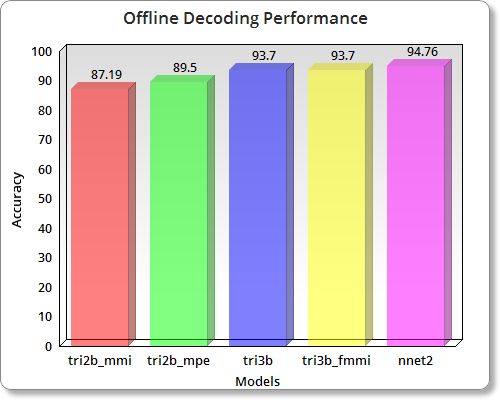
\includegraphics[width=13cm, height=8cm]{./img/Models}}
 \caption{GMM-HMM models}
\label{fig:Models}
\end{figure}

Here we trained the models with 9324 utterances of 1035 isolated words and the total number of different speakers is 91 where the number of male and female speakers is 62 and 29.
Where we have got so far good result using the new B-ToBI model of Bengali intonation \cite{khan2016intonation}.

\section{Comparison of previous DNN-HMM models}
This section is about the comparison of previous DNN-HMM models and our model accuracy.
Finally, we have got better accuracy in using the Kaldi's DNN-HMM model with a large corpus and different male-female ratio.
\\
\begin{figure}[H]
 \centering
 \frame{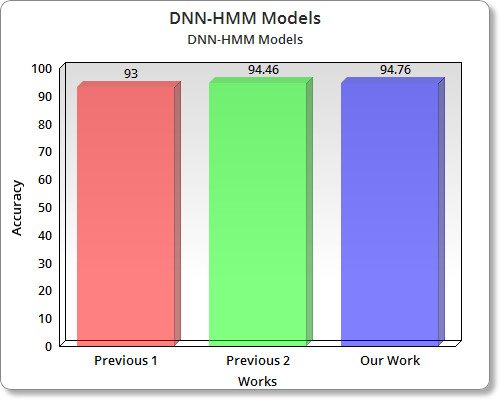
\includegraphics[width=13cm, height=8cm]{./img/DNN-HMM_comparison}}
 \caption{Comparison of previous DNN-HMM models}
\label{fig:DNN-HMM_comparison}
\end{figure}




\end{document}